\documentclass[12pt,openany]{book}
\usepackage[a4paper,margin=1in]{geometry}
\usepackage{amsmath,amsthm,amssymb}
\usepackage{tikz}
\usepackage{forest}
\usepackage[hidelinks]{hyperref}
\usepackage{listings}
\usepackage{graphicx}
\usepackage{fancyhdr}
\usepackage{algorithm}
\usepackage{algpseudocode}
\pagestyle{fancy}
\fancyhf{}
\fancyfoot[C]{\thepage}
\renewcommand{\headrulewidth}{0pt}
\usepackage{titlesec}
\titleformat{\chapter}[hang]{\normalfont\huge\bfseries}{\thechapter}{1em}{}

\title{Modular Arithmetic}
\author{Beulah Evanjalin}
\date{}

\theoremstyle{definition}
\newtheorem{definition}{Definition}[chapter]
\newtheorem{example}{Example}[chapter]
\theoremstyle{plain}
\newtheorem{theorem}{Theorem}[chapter]
\newtheorem{proposition}{Proposition}[chapter]
\newtheorem{corollary}{Corollary}[chapter]
\newtheorem{lemma}{Lemma}[chapter]
\theoremstyle{remark}
\newtheorem{remark}{Remark}[chapter]

\begin{document}
\maketitle
\tableofcontents

\chapter{Introduction}

Modular arithmetic, often referred to as \emph{clock arithmetic}, is a foundational tool in mathematics, particularly when working within finite algebraic structures.
\\ \\
Modular arithmetic concerns operations within the ring of integers modulo $m$, denoted $\mathbb{Z}/m\mathbb{Z}$, where arithmetic is performed under the equivalence relation $a \equiv b \pmod{m}$. This equivalence partitions the integers into congruence classes, facilitating operations where values are periodically identified.

\section{Applications}

Many public-key cryptographic protocols rely intrinsically on modular arithmetic due to its favorable computational properties and algebraic hardness assumptions.

\begin{itemize}
  \item \textbf{RSA Cryptosystem}: Based on Euler's theorem, RSA operates with a modulus $n = pq$, where $p$ and $q$ are large primes. Given $e$ such that $\gcd(e, \phi(n)) = 1$, encryption is given by $c \equiv m^e \pmod{n}$, and decryption via $m \equiv c^d \pmod{n}$, where $d \equiv e^{-1} \pmod{\phi(n)}$.

  \item \textbf{Diffie-Hellman Key Exchange}: Employs modular exponentiation in a finite cyclic group $\mathbb{Z}_p^*$, enabling secure computation of shared secrets over insecure channels by leveraging the discrete logarithm problem.

  \item \textbf{Elliptic Curve Cryptography (ECC)}: Extends modular arithmetic to elliptic curves over finite fields $\mathbb{F}_p$ or $\mathbb{F}_{2^m}$, offering higher cryptographic strength per bit through richer group structures.
\end{itemize}
\noindent
Note: In each of these above schemes, the feasibility of operations like $a^b \bmod m$ for very large integers requires efficient exponentiation algorithms, such as binary exponentiation (a.k.a. square-and-multiply).
\begin{itemize}
  \item \textbf{Hash Functions}: Use modular reduction to constrain outputs to a fixed-size range, as seen in hash tables and cryptographic digests.
  \item \textbf{Random Number Generators}: Pseudorandom sequences, such as those from linear congruential generators, are defined recursively as $x_{n+1} \equiv ax_n + c \pmod{m}$.
  \item \textbf{Finite Field Arithmetic}: Key to error-correcting codes like \href{https://en.wikipedia.org/wiki/Reed%E2%80%93Solomon_error_correction}{Reed-Solomon}, which operate over $\mathbb{F}_q$, often implemented using modular arithmetic over prime fields.
  \item \textbf{Big Integer Libraries}: Efficient handling of arithmetic with large numbers often requires modular reductions to manage intermediate computations and memory usage.
\end{itemize}

\section{Role in Number Theory}
Within mathematics, modular arithmetic provides both a practical tool and a conceptual framework:
\begin{itemize}
  \item \textbf{Fermat's Last Theorem}: \href{https://en.wikipedia.org/wiki/Wiles%27s_proof_of_Fermat%27s_Last_Theorem}{Wiles' proof} is based on modular forms and elliptic curves, where congruence relations play a central role.
  \item \textbf{Distribution of Primes}: Properties such as Dirichlet’s theorem on arithmetic progressions and the properties of residues mod $n$ shape analytic and algebraic number theory.
  \item \textbf{Solving Diophantine Equations}: Modulo constraints reduce complex integer problems to manageable local conditions, facilitating techniques like Hensel’s lemma and the method of descent.
\end{itemize}

Abstractly, modular systems exemplify rings, fields (when modulus is prime), and groups, which provide concrete cases for studying general algebraic structures.

\section{Historical Origins}

Although modular arithmetic was formalized in the 19\textsuperscript{th} century, its roots extend to antiquity.

\begin{itemize}
  \item \textbf{Early Chinese Mathematics}: \emph{Sunzi Suanjing} (circa 100 BCE) outlines problems equivalent to the modern Chinese Remainder Theorem (CRT). For example, solving:
  \[
    \begin{cases}
      x \equiv 2 \pmod{3} \\
      x \equiv 3 \pmod{5} \\
      x \equiv 2 \pmod{7}
    \end{cases}
  \]
  yields $x \equiv 23 \pmod{105}$, showcasing congruential reasoning.

  \item \textbf{Gauss (1801)}: In \emph{Disquisitiones Arithmeticae}, Gauss introduced the formal congruence notation $a \equiv b \pmod{m}$, established properties such as the law of quadratic reciprocity, and laid the foundation for modern number theory.

  \item \textbf{Euler and Fermat}: Fermat’s Little Theorem and Euler’s generalization via the totient function $\phi(n)$ demonstrated the periodic nature of powers modulo primes and composites, which is fundamental to later cryptographic applications.

  \item \textbf{Computational Era}: In the mid 20\textsuperscript{th} century, there was a need for more efficient algorithms, such as exponentiation by squaring. By the 1970s, cryptographic primitives like RSA and ElGamal leveraged modular arithmetic for secure digital communication.

  \item \textbf{Quantum and Post-Quantum}: Even in the face of quantum algorithms (e.g., Shor's), many post-quantum cryptographic schemes retain modular structures in lattice-based and code-based cryptography, indicating its enduring utility.
\end{itemize}



\chapter{Basics of Congruences}
\begin{definition}
  Let $m \geq 1$ be an integer (the \textbf{modulus}). We say that two integers $a$ and $b$ are \textbf{congruent modulo $m$}, denoted $a \equiv b \pmod{m}$, if $m$ divides $a - b$, i.e., $m \mid (a - b)$.
\end{definition}
\noindent
Equivalently, there exists an integer $k$ such that $a = b + k m$. This relation captures the notion of ``remainder" when dividing by $m$: $a$ and $b$ leave the same remainder upon division by $m$.

\begin{example}\mbox{}\\[-0.8em]
  \begin{itemize}
    \item $15 \equiv 3 \pmod{12}$ because $15 - 3 = 12$, and $12 \mid 12$.
    \item $-1 \equiv 11 \pmod{12}$ because $-1 - 11 = -12$, and $12 \mid -12$.
    \item $17 \equiv 2 \pmod{5}$ because $17 = 3 \cdot 5 + 2$, so $17 - 2 = 15$, and $5 \mid 15$.
    \item However, $19 \not\equiv 6 \pmod{11}$ because $19 - 6 = 13$, and $11 \nmid 13$.
  \end{itemize}
\end{example}

\section{Equivalence Relation}

Congruence modulo $m$ defines an equivalence relation on the set of integers $\mathbb{Z}$, partitioning it into disjoint classes.

\begin{theorem}
  Congruence modulo $m$ is an equivalence relation on $\mathbb{Z}$, satisfying:
  \begin{itemize}
    \item \textbf{Reflexivity}: $a \equiv a \pmod{m}$ for all $a \in \mathbb{Z}$.
    \item \textbf{Symmetry}: If $a \equiv b \pmod{m}$, then $b \equiv a \pmod{m}$.
    \item \textbf{Transitivity}: If $a \equiv b \pmod{m}$ and $b \equiv c \pmod{m}$, then $a \equiv c \pmod{m}$.
  \end{itemize}
\end{theorem}

\begin{proof}\mbox{}\\[-0.8em]
  \begin{itemize}
    \item \textbf{Reflexivity}: $a - a = 0$, and $m \mid 0$ (since $0 = m \cdot 0$).
    \item \textbf{Symmetry}: If $m \mid (a - b)$, then $a - b = k m$ for some integer $k$, so $b - a = (-k) m$, hence $m \mid (b - a)$.
    \item \textbf{Transitivity}: If $m \mid (a - b)$ and $m \mid (b - c)$, then $a - b = k m$ and $b - c = l m$ for integers $k, l$. Thus, $a - c = (a - b) + (b - c) = (k + l) m$, so $m \mid (a - c)$.
  \end{itemize}
\end{proof}

\section{Residue Classes}
This equivalence relation partitions $\mathbb{Z}$ into $m$ distinct \textbf{residue classes} (or \textbf{congruence classes}).

\begin{definition}
  The \textbf{residue class} of $a$ modulo $m$ is the set
  \[
    [a]_m = \{ b \in \mathbb{Z} : b \equiv a \pmod{m} \} = \{ a + k m : k \in \mathbb{Z} \}.
  \]
  The set of all residue classes modulo $m$ is denoted $\mathbb{Z}/m\mathbb{Z}$.
\end{definition}
\noindent
There are exactly $m$ distinct residue classes, which can be represented by the remainders $0, 1, \dots, m-1$ when dividing by $m$. For any integer $a$, we can write $a = q m + r$ with $0 \leq r < m$ (by the Division Algorithm), so $[a]_m = [r]_m$.

\begin{example}
  For $m=5$, the residue classes are:
  \begin{itemize}
    \item $[0]_5 = \{\dots, -10, -5, 0, 5, 10, \dots\}$
    \item $[1]_5 = \{\dots, -9, -4, 1, 6, 11, \dots\}$
    \item $[2]_5 = \{\dots, -8, -3, 2, 7, 12, \dots\}$
    \item $[3]_5 = \{\dots, -7, -2, 3, 8, 13, \dots\}$
    \item $[4]_5 = \{\dots, -6, -1, 4, 9, 14, \dots\}$
  \end{itemize}
  Note that $17 \equiv 2 \pmod{5}$, so $[17]_5 = [2]_5$.
\end{example}

\section{Arithmetic of Congruences}

Congruences behave similarly to equalities under addition, subtraction, and multiplication.

\begin{proposition}
  If $a_1 \equiv a_2 \pmod{m}$ and $b_1 \equiv b_2 \pmod{m}$, then
  \[
    a_1 + b_1 \equiv a_2 + b_2 \pmod{m}, \quad a_1 - b_1 \equiv a_2 - b_2 \pmod{m}, \quad a_1 b_1 \equiv a_2 b_2 \pmod{m}.
  \]
\end{proposition}

\begin{proof}
  Since $a_1 \equiv a_2 \pmod{m}$, we have $a_1 = a_2 + k m$ for some integer $k$. Similarly, $b_1 = b_2 + l m$ for some $l$.
  \begin{itemize}
    \item Addition: $a_1 + b_1 = (a_2 + b_2) + (k + l) m$, so $m \mid [(a_1 + b_1) - (a_2 + b_2)]$.
    \item Subtraction: $a_1 - b_1 = (a_2 - b_2) + (k - l) m$, so $m \mid [(a_1 - b_1) - (a_2 - b_2)]$.
    \item Multiplication: $a_1 b_1 = (a_2 + k m)(b_2 + l m) = a_2 b_2 + a_2 (l m) + b_2 (k m) + (k l) m^2 = a_2 b_2 + m (a_2 l + b_2 k + k l m)$, so $m \mid (a_1 b_1 - a_2 b_2)$.
  \end{itemize}
\end{proof}

\begin{corollary}
  If $a \equiv b \pmod{m}$, then for any integer $k \geq 0$, $a^k \equiv b^k \pmod{m}$.
\end{corollary}

\begin{proof}
  By induction on $k$. Base: $k=0$, $1 \equiv 1$. Assume for $k-1$: $a^{k-1} \equiv b^{k-1} \pmod{m}$. Then $a^k = a \cdot a^{k-1} \equiv b \cdot b^{k-1} = b^k \pmod{m}$.
\end{proof}

\begin{example}\subsubsection*{}
  Compute $6 + 9 \pmod{12}$: $6 + 9 = 15 \equiv 3 \pmod{12}$. Alternatively, $6 \equiv 18 \pmod{12}$, $9 \equiv -3 \pmod{12}$, so $18 + (-3) = 15 \equiv 3 \pmod{12}$.
\noindent
\\ \\
  For multiplication: $2 \cdot 3 = 6 \equiv 1 \pmod{5}$, since $2 \equiv 7 \pmod{5}$, $3 \equiv 8 \pmod{5}$, $7 \cdot 8 = 56 \equiv 1 \pmod{5}$ (as $55 = 11 \cdot 5$).
\end{example}
\noindent
These properties allow us to perform arithmetic ``modulo $m$" by reducing intermediates.

\section{Cancellation and Division}

Division in modular arithmetic is subtle and requires care, often involving multiplicative inverses. However, a cancellation law holds under certain conditions.

\begin{proposition}
  If $a c \equiv b c \pmod{m}$ and $d = \gcd(c, m)$, then $a \equiv b \pmod{m/d}$.
\end{proposition}

\begin{proof}
  Given $a c \equiv b c \pmod{m}$, we have $m \mid (a c - b c) = c (a - b)$. Let $d = \gcd(c, m)$. Write $c = d c'$, $m = d m'$ with $\gcd(c', m') = 1$. Then $d m' \mid d c' (a - b)$, so $m' \mid c' (a - b)$. Since $\gcd(c', m') = 1$, it follows that $m' \mid (a - b)$ (by Euclid's lemma), hence $a \equiv b \pmod{m' = m/d}$.
\end{proof}

\begin{corollary}
  If $\gcd(c, m) = 1$, then $a c \equiv b c \pmod{m}$ implies $a \equiv b \pmod{m}$.
\end{corollary}

\begin{example}\subsubsection*{}
  Suppose $4x \equiv 12 \pmod{10}$. Here $c = 4$, $m = 10$, and $\gcd(4, 10) = 2$. According to the cancellation proposition, we can divide both sides of the congruence by $d = 2$, provided we reduce the modulus accordingly. That is, the solutions satisfy:
  \[
    x \equiv \frac{12}{2} \cdot (4/2)^{-1} \pmod{10/2} \quad \Rightarrow \quad x \equiv 6 \cdot 2^{-1} \pmod{5}
  \]
  Since $2^{-1} \equiv 3 \pmod{5}$ (because $2 \cdot 3 = 6 \equiv 1 \pmod{5}$), we get:
  \[
    x \equiv 6 \cdot 3 = 18 \equiv 3 \pmod{5}
  \]
  So $x \equiv 3 \pmod{5}$ is the solution set.
  \medskip
  \noindent
  \\
  Verification: choose $x = 3$, then $4x = 12 \equiv 2 \pmod{10}$. Wait! this doesn't match the original equation $4x \equiv 12 \pmod{10}$, because $12 \equiv 2 \pmod{10}$, so this suggests a mistake.
  \noindent
  \\
  Actually, we need to reframe the initial congruence correctly: since $4x \equiv 12 \pmod{10}$ and $12 \equiv 2 \pmod{10}$, the congruence is really:
  \[
    4x \equiv 2 \pmod{10}
  \]
  Now apply the proposition: $\gcd(4, 10) = 2$ divides $2$, so we can divide throughout by $2$ to get:
  \[
    2x \equiv 1 \pmod{5}
  \]
  The inverse of $2$ modulo $5$ is $3$ (since $2 \cdot 3 = 6 \equiv 1 \pmod{5}$), so:
  \[
    x \equiv 3 \pmod{5}
  \]

  \medskip
  \noindent
  \\
  Let's verify with $x = 3$:
  \[
    4x = 12 \equiv 2 \pmod{10} \quad \text{correct}.
  \]
  \medskip
  \noindent
  \\
  Now, consider a case where $\gcd = 1$, such as $3x \equiv 6 \pmod{7}$. Since $\gcd(3, 7) = 1$, we can directly multiply both sides by the inverse of $3$ modulo $7$. Since $3^{-1} \equiv 5 \pmod{7}$ (because $3 \cdot 5 = 15 \equiv 1 \pmod{7}$), we get:
  \[
    x \equiv 5 \cdot 6 = 30 \equiv 2 \pmod{7}
  \]
  \noindent
  \\
  Verified: $3 \cdot 2 = 6 \equiv 6 \pmod{7}$ \text{correct}.
\end{example}
\noindent
\\
Note that if $\gcd(c,m)>1$, cancellation may not hold modulo $m$, but only modulo $m/d$. This highlights why inverses exist only when coprime.



\chapter{The Ring $\mathbb{Z}/m\mathbb{Z}$}

Building on the concept of congruences from the previous section, we now formalize the algebraic structure formed by the residue classes modulo $m$. This structure, denoted $\mathbb{Z}/m\mathbb{Z}$, is a fundamental object in abstract algebra and number theory, serving as a prototype for finite rings and fields.

\section{Construction and Ring Axioms}

The set $\mathbb{Z}/m\mathbb{Z}$ consists of the $m$ distinct residue classes modulo $m$:
\[
\mathbb{Z}/m\mathbb{Z} = \{ [0]_m, [1]_m, \dots, [m-1]_m \},
\]
where $[a]_m = \{ b \in \mathbb{Z} : b \equiv a \pmod{m} \}$.
\noindent
\\ \\
To make $\mathbb{Z}/m\mathbb{Z}$ into a ring, we define addition and multiplication on these classes:
\[
[a]_m + [b]_m = [a + b]_m, \quad [a]_m \cdot [b]_m = [a b]_m.
\]
\noindent
\\
These operations are \textbf{well-defined}, meaning they do not depend on the choice of representatives. If $[a'] = [a]$ and $[b'] = [b]$, then $a' \equiv a \pmod{m}$ and $b' \equiv b \pmod{m}$, so $a' + b' \equiv a + b \pmod{m}$ and $a' b' \equiv a b \pmod{m}$ by the arithmetic properties of congruences.

\begin{theorem}
  $(\mathbb{Z}/m\mathbb{Z}, +, \cdot)$ is a commutative ring with identity.
\end{theorem}

\begin{proof}
  The ring axioms are satisfied as follows:
  \begin{itemize}
    \item \textbf{Addition is associative and commutative}: Inherited from $\mathbb{Z}$, e.g., $([a] + [b]) + [c] = [a + b + c] = [a] + ([b] + [c])$.
    \item \textbf{Additive identity}: $[0]$, since $[a] + [0] = [a]$.
    \item \textbf{Additive inverses}: For $[a]$, the inverse is $[-a]$, since $[a] + [-a] = [0]$.
    \item \textbf{Multiplication is associative and commutative}: Similarly from $\mathbb{Z}$.
    \item \textbf{Multiplicative identity}: $[1]$, since $[a] \cdot [1] = [a]$.
    \item \textbf{Distributivity}: $[a] \cdot ([b] + [c]) = [a(b + c)] = [a b + a c] = [a b] + [a c] = [a] \cdot [b] + [a] \cdot [c]$.
  \end{itemize}
  Commutativity of both operations follows from $\mathbb{Z}$.
\end{proof}

\begin{example}
  For $m=5$, addition and multiplication tables in $\mathbb{Z}/5\mathbb{Z}$ are:
  \noindent
  \\ \\
  \textbf{Addition Table:}
  \begin{center}
    \begin{tabular}{c|ccccc}
      + & 0 & 1 & 2 & 3 & 4 \\ \hline
      0 & 0 & 1 & 2 & 3 & 4 \\
      1 & 1 & 2 & 3 & 4 & 0 \\
      2 & 2 & 3 & 4 & 0 & 1 \\
      3 & 3 & 4 & 0 & 1 & 2 \\
      4 & 4 & 0 & 1 & 2 & 3 \\
    \end{tabular}
  \end{center}
  \noindent
  \\ \\
  \textbf{Multiplication Table:}
  \begin{center}
    \begin{tabular}{c|ccccc}
      $\cdot$ & 0 & 1 & 2 & 3 & 4 \\ \hline
      0 & 0 & 0 & 0 & 0 & 0 \\
      1 & 0 & 1 & 2 & 3 & 4 \\
      2 & 0 & 2 & 4 & 1 & 3 \\
      3 & 0 & 3 & 1 & 4 & 2 \\
      4 & 0 & 4 & 3 & 2 & 1 \\
    \end{tabular}
  \end{center}
\end{example}
\noindent
\\ \\
$\mathbb{Z}/m\mathbb{Z}$ is the \textbf{quotient ring} of $\mathbb{Z}$ by the ideal $m\mathbb{Z}$.

\section{Units and Zero Divisors}

Not every non-zero element in $\mathbb{Z}/m\mathbb{Z}$ has a multiplicative inverse, leading to the distinction between units and zero divisors.

\begin{definition}
  An element $[a] \in \mathbb{Z}/m\mathbb{Z}$ is a \textbf{unit} if there exists $[b]$ such that $[a] \cdot [b] = [1]$. The set of units is
  \[
  (\mathbb{Z}/m\mathbb{Z})^* = \{ [a] \in \mathbb{Z}/m\mathbb{Z} : \gcd(a, m) = 1 \}.
  \]
\end{definition}

\begin{proposition}
  $[a]$ is a unit if and only if $\gcd(a, m) = 1$.
\end{proposition}

\begin{proof}
  If $\gcd(a, m) = 1$, by Bézout's identity (later chapter), there exist integers $u, v$ with $a u + m v = 1$, so $[a] [u] = [1]$. Conversely, if $[a] [b] = [1]$, then $a b \equiv 1 \pmod{m}$, so $\gcd(a, m)$ divides 1.
\end{proof}
\noindent
$(\mathbb{Z}/m\mathbb{Z})^*$ forms a group under multiplication.

\begin{definition}
  A non-zero element $[a]$ is a \textbf{zero divisor} if there exists non-zero $[b]$ with $[a] [b] = [0]$.
\end{definition}

\begin{proposition}
  $[a] \neq [0]$ is a zero divisor if and only if $\gcd(a, m) > 1$.
\end{proposition}

\begin{proof}
  ($\Rightarrow$) Suppose $\gcd(a, m) = 1$; then $[a]$ is a unit, so if $[a] [b] = [0]$, multiply by inverse: $[b] = [0]$, contradiction.  
  ($\Leftarrow$) Let $d = \gcd(a, m) > 1$, $a = d a'$, $m = d m'$ with $\gcd(a', m') = 1$. Then $[a] [m'] = [d a' m'] = [a' m] = [0]$, and $[m'] \neq [0]$ since $m' < m$.
\end{proof}

\begin{example}
  In $\mathbb{Z}/6\mathbb{Z}$, units are $\{[1], [5]\}$ ($\gcd(1,6)=1$, $\gcd(5,6)=1$). Zero divisors: $[2]$ ($\gcd(2,6)=2>1$, $[2][3]=[6]=[0]$), $[3]$ ($\gcd(3,6)=3>1$), $[4]$ ($\gcd(4,6)=2>1$).
\end{example}

\section{Field Structure for Prime Modulus}

When $m = p$ is prime, $\mathbb{Z}/p\mathbb{Z}$ has additional structure.

\begin{theorem}
  If $p$ is prime, then $\mathbb{Z}/p\mathbb{Z}$ is a field.
\end{theorem}

\begin{proof}
  Every non-zero $[a]$ has $\gcd(a, p) = 1$ (since $p$ is prime and doesn't divide $a$), so all non-zero elements are units. There are no zero divisors (as that would require $\gcd(a, p) > 1$, impossible for $a \not\equiv 0$). Thus, it satisfies the field axioms: it's a commutative ring with identity where every non-zero element has an inverse.
\end{proof}
\noindent
Fields like $\mathbb{Z}/p\mathbb{Z}$ (denoted $\mathbb{F}_p$) are crucial for finite field arithmetic in cryptography and coding theory.

\begin{example}
  $\mathbb{Z}/5\mathbb{Z}$ is a field: every non-zero element has an inverse, e.g., $[2]^{-1} = [3]$ since $2 \cdot 3 = 6 \equiv 1 \pmod{5}$.
\end{example}

\section{Euler’s Phi Function}

To quantify the units, we introduce Euler's totient function.

\begin{definition}
  Euler's \textbf{phi function} (totient function) is
  \[
  \phi(m) = |(\mathbb{Z}/m\mathbb{Z})^*| = \#\{ a : 1 \leq a \leq m, \gcd(a, m) = 1 \}.
  \]
\end{definition}

\begin{example}
  \begin{itemize}
    \item $\phi(7) = 6$ (all 1 through 6 are coprime to 7).
    \item $\phi(24) = 8$ (1,5,7,11,13,17,19,23).
  \end{itemize}
\end{example}

\begin{theorem}[Euler's Product Formula]
  If $m = p_1^{k_1} \cdots p_r^{k_r}$, then
  \[
  \phi(m) = m \prod_{i=1}^r \left(1 - \frac{1}{p_i}\right) = \prod_{i=1}^r p_i^{k_i - 1} (p_i - 1).
  \]
\end{theorem}

\begin{proof}
  For prime power $p^k$, $\phi(p^k) = p^k - p^{k-1}$ (subtract multiples of $p$). The general case follows from multiplicativity (below).
\end{proof}

\begin{theorem}[Multiplicativity]
  If $\gcd(m, n) = 1$, then $\phi(m n) = \phi(m) \phi(n)$.
\end{theorem}

\begin{proof}
  By the Chinese Remainder Theorem (later chapter), there is a ring isomorphism $\mathbb{Z}/(m n)\mathbb{Z} \cong \mathbb{Z}/m\mathbb{Z} \times \mathbb{Z}/n\mathbb{Z}$, which restricts to a group isomorphism $(\mathbb{Z}/(m n)\mathbb{Z})^* \cong (\mathbb{Z}/m\mathbb{Z})^* \times (\mathbb{Z}/n\mathbb{Z})^*$. Thus, the orders multiply: $\phi(m n) = \phi(m) \phi(n)$.
\end{proof}
\noindent
\\
$\phi(m)$ counts integers up to $m$ coprime to $m$ and is key in Euler's theorem.


\chapter{Extended Euclidean Algorithm \& Inverses}

The Euclidean algorithm and its extended form are essential tools in number theory for computing greatest common divisors (GCDs) and solving linear Diophantine equations. These algorithms are particularly useful in modular arithmetic for finding multiplicative inverses, which are crucial for division modulo $m$ and applications in cryptography.

\section{Euclidean Algorithm}

The Euclidean algorithm efficiently computes the greatest common divisor $\gcd(a, b)$ of two integers $a$ and $b$ (assume $a \geq b > 0$ without loss of generality). It is based on the principle that $\gcd(a, b) = \gcd(b, a \mod b)$, repeatedly replacing the larger number with the remainder until a remainder of zero is reached.

\begin{definition}
  The \textbf{greatest common divisor} $\gcd(a, b)$ is the largest positive integer $d$ that divides both $a$ and $b$.
\end{definition}

\begin{algorithm}[H]
\caption{Euclidean Algorithm}
\begin{algorithmic}[1]
\Require Integers $a \geq b > 0$
\Ensure $\gcd(a, b)$
\While{$b \ne 0$}
  \State $q \gets \lfloor a / b \rfloor$ \Comment{quotient}
  \State $r \gets a - q b$ \Comment{remainder}
  \State $a \gets b$
  \State $b \gets r$
\EndWhile
\State \Return $a$
\end{algorithmic}
\end{algorithm}


\begin{example}
  Compute $\gcd(252, 105)$:
  \begin{align*}
    252 &= 2 \cdot 105 + 42, \\
    105 &= 2 \cdot 42 + 21, \\
    42 &= 2 \cdot 21 + 0.
  \end{align*}
  So $\gcd(252, 105) = 21$.
\end{example}

\newpage

\begin{theorem}[Correctness of Euclidean Algorithm]
  The algorithm computes $\gcd(a, b)$ in $O(\log \min(a, b))$ steps.
\end{theorem}

\begin{proof}\*subsubsection{}
  Let $r_0 = a$, $r_1 = b$, and define $r_{i+1} = r_{i-1} \mod r_i$. The sequence of remainders is strictly decreasing and non-negative: $r_{i+1} < r_i$. It terminates when $r_k = 0$, and $\gcd(a, b) = r_{k-1}$.
  \noindent
  \\ \\
  To show correctness: Any common divisor of $a$ and $b$ divides all remainders (since $r_{i+1} = r_{i-1} - q_i r_i$). Conversely, working backwards, any divisor of the final non-zero remainder divides $a$ and $b$. Thus, $\gcd(a, b) = r_{k-1}$.
  \noindent
  \\ \\
  For complexity: Each step reduces the remainder by at least half in the worst case (Fibonacci numbers), leading to $O(\log \min(a, b))$.
\end{proof}

\section{Extended Algorithm}

The extended Euclidean algorithm augments the basic algorithm to find integers $u$ and $v$ satisfying Bézout's identity.

\begin{algorithm}[H]
\caption{Extended Euclidean Algorithm}
\begin{algorithmic}[1]
\Require Integers $a, b$
\Ensure $d = \gcd(a, b)$, and $u, v$ such that $a u + b v = d$
\State $u \gets 1$, $v \gets 0$
\State $u' \gets 0$, $v' \gets 1$
\While{$b \ne 0$}
  \State $q \gets \lfloor a / b \rfloor$
  \State $r \gets a - q \cdot b$
  \State $u'' \gets u - q \cdot u'$
  \State $v'' \gets v - q \cdot v'$
  \State $a \gets b$, $b \gets r$
  \State $u \gets u'$, $v \gets v'$
  \State $u' \gets u''$, $v' \gets v''$
\EndWhile
\State \Return $d = a$, $u$, $v$
\end{algorithmic}
\end{algorithm}
\noindent
This tracks coefficients $u$ and $v$ through the remainders.
\\
\begin{theorem}[Bézout's Identity]
  For any integers $a, b$, there exist integers $u, v$ such that $a u + b v = \gcd(a, b)$.
\end{theorem}

\begin{proof}
  The proof is by induction on the steps of the Euclidean algorithm. Base case: If $b = 0$, then $\gcd(a, 0) = |a|$, and $a \cdot 1 + 0 \cdot 0 = a$ (adjust sign if needed).
  \noindent
  \\ \\
  Inductive step: Assume for smaller pairs. From $a = q b + r$, $\gcd(a, b) = \gcd(b, r)$. By induction, $b u' + r v' = \gcd(b, r)$. Substitute $r = a - q b$: $b u' + (a - q b) v' = a v' + b (u' - q v') = \gcd(a, b)$. Thus $u = v'$, $v = u' - q v'$.
  \noindent
  \\ \\
  The extended algorithm implements this back-substitution efficiently.
\end{proof}

\begin{example}\subsubsection*{}
  For $a = 252$, $b = 105$:
  \begin{align*}
    252 &= 2 \cdot 105 + 42 \\
    105 &= 2 \cdot 42 + 21 \\
     42 &= 2 \cdot 21 + 0
  \end{align*}
  So $\gcd(252, 105) = 21$.
  \medskip
  Now back-substituting to express $21$ as a linear combination of $252$ and $105$:
  \begin{align*}
    21 &= 105 - 2 \cdot 42 \\
       &= 105 - 2 \cdot (252 - 2 \cdot 105) \\
       &= 105 - 2 \cdot 252 + 4 \cdot 105 \\
       &= (-2) \cdot 252 + 5 \cdot 105
  \end{align*}
  \medskip
  Therefore, $252 \cdot (-2) + 105 \cdot 5 = 21 = \gcd(252, 105)$.
\end{example}
\noindent
The algorithm runs in $O(\log \min(a, b))$ time, same as the basic version.

\section{Computing Multiplicative Inverse}

If $\gcd(a, m) = 1$, $a$ has a multiplicative inverse modulo $m$: an integer $u$ such that $a u \equiv 1 \pmod{m}$. This $u$ is unique modulo $m$.
\noindent
\\ \\
From Bézout: $a u + m v = 1$, so $a u \equiv 1 \pmod{m}$.

\begin{algorithm}[H]
\caption{Modular Inverse via Extended Euclidean}
\begin{algorithmic}[1]
\Require $a, m$ with $\gcd(a, m) = 1$.
\Ensure $u$ such that $a u \equiv 1 \pmod{m}$.
\State Use extended Euclidean on $a, m$ to get $u, v$ with $a u + m v = 1$.
\Return $u \mod m$ (adjust to positive if needed).
\end{algorithmic}
\end{algorithm}

\begin{example}
  Find the inverse of 5 modulo 12 (since $\gcd(5, 12) = 1$).
  \noindent
  \\
  Apply Euclidean algorithm:
  \begin{align*}
    12 &= 2 \cdot 5 + 2, \\
    5 &= 2 \cdot 2 + 1, \\
    2 &= 2 \cdot 1 + 0.
  \end{align*}
  \noindent
  \\
  Back-substitution:
  \begin{align*}
    1 &= 5 - 2 \cdot 2, \\
    2 &= 12 - 2 \cdot 5, \\
    1 &= 5 - 2 \cdot (12 - 2 \cdot 5) = 5 - 2 \cdot 12 + 4 \cdot 5 = 5 \cdot 5 - 2 \cdot 12.
  \end{align*}
  \noindent
  \\
  Thus, $5 \cdot 5 \equiv 1 \pmod{12}$, so the inverse is $5 \mod 12 = 5$. Verify: $5 \cdot 5 = 25 \equiv 1 \pmod{12}$.
\end{example}

\begin{example}
  Inverse of 11 modulo 26:
  \begin{align*}
    26 &= 2 \cdot 11 + 4, \\
    11 &= 2 \cdot 4 + 3, \\
    4 &= 1 \cdot 3 + 1, \\
    3 &= 3 \cdot 1 + 0.
  \end{align*}
  \noindent
  \\
  Back-substitution:
  \begin{align*}
    1 &= 4 - 1 \cdot 3, \\
    3 &= 11 - 2 \cdot 4, \quad 1 &= 4 - 1 \cdot (11 - 2 \cdot 4) = 3 \cdot 4 - 1 \cdot 11, \\
    4 &= 26 - 2 \cdot 11, \quad 1 &= 3 \cdot (26 - 2 \cdot 11) - 1 \cdot 11 = 3 \cdot 26 - 7 \cdot 11.
  \end{align*}
  \noindent
  \\
  So $11 \cdot (-7) \equiv 1 \pmod{26}$, and $-7 \equiv 19 \pmod{26}$. Verify: $11 \cdot 19 = 209 = 8 \cdot 26 + 1 \equiv 1 \pmod{26}$.
\end{example}
\noindent
\\
If $\gcd(a, m) \neq 1$, no inverse exists.
\noindent
\\ \\
This method is efficient, requiring $O(\log m)$ steps, vital for cryptographic computations.

\chapter{Euler’s Theorem and Applications}

This section brings together the key results of Euler and Fermat, which underpin much of modern public-key cryptography, and demonstrates practical applications in fundamental cryptosystems.

\section{Euler’s Theorem}

\begin{theorem}[Euler’s Theorem]
  Let $m \geq 1$ and let $a$ be an integer with $\gcd(a, m) = 1$. Then
  \[
    a^{\varphi(m)} \equiv 1 \pmod{m},
  \]
  where $\varphi(m)$ is Euler’s totient function, the number of integers $1 \leq k \leq m$ that are coprime to $m$.
\end{theorem}

\begin{proof}
  The set of invertible elements modulo $m$ forms a multiplicative group of order $\varphi(m)$, namely $(\mathbb{Z}/m\mathbb{Z})^* = \{ [b] : 1 \leq b \leq m, \gcd(b, m) = 1 \}$. By Lagrange’s theorem (from group theory), for any $[a]$ in this group,
  \[
    [a]^{\varphi(m)} = [1],
  \]
  which means $a^{\varphi(m)} \equiv 1 \pmod{m}$.
\end{proof}

\section{Fermat’s Little Theorem}

As a special case of Euler’s theorem, we have:

\begin{theorem}[Fermat’s Little Theorem]
  Let $p$ be a prime. For any integer $a$ not divisible by $p$,
  \[
    a^{p-1} \equiv 1 \pmod{p}.
  \]
\end{theorem}

\begin{proof}
  For $p$ prime, $\varphi(p) = p-1$, so Euler’s theorem applies directly: $a^{p-1} \equiv 1 \pmod{p}$ for $a \not\equiv 0 \pmod{p}$.
\end{proof}

\newpage

\section{Applications to Cryptography}

Modular exponentiation theorems such as those of Euler and Fermat are the working engine inside multiple cryptosystems. We highlight two:

\begin{itemize}
  \item \textbf{RSA Cryptosystem:}
    \begin{itemize}
      \item \emph{Key Generation:} Choose distinct large primes $p$, $q$; let $n = pq$, compute $\varphi(n) = (p-1)(q-1)$.
      \item \emph{Public Key:} $(n, e)$ such that $1 < e < \varphi(n)$ and $\gcd(e, \varphi(n)) = 1$.
      \item \emph{Private Key:} $d$ satisfying $e d \equiv 1 \pmod{\varphi(n)}$ (computed using the Extended Euclidean Algorithm).
      \item \emph{Encryption:} $c \equiv m^e \pmod{n}$.
      \item \emph{Decryption:} $m \equiv c^d \pmod{n}$.
      \item \emph{Correctness:} As $ed \equiv 1 \pmod{\varphi(n)}$ and $\gcd(m, n)=1$, Euler’s theorem gives $m^{\varphi(n)} \equiv 1 \pmod{n}$, so $(m^e)^d \equiv m \pmod{n}$.
    \end{itemize}
  \item \textbf{Diffie–Hellman Key Exchange:}
    \begin{itemize}
      \item Parties agree on a prime $p$ and generator $g$ of $(\mathbb{Z}/p\mathbb{Z})^*$.
      \item Alice selects secret $a$ and sends $A = g^a \pmod{p}$; Bob selects secret $b$ and sends $B = g^b \pmod{p}$.
      \item Alice computes $k = B^a \pmod{p}$; Bob computes $k = A^b \pmod{p}$.
      \item By commutativity, $k = g^{ab} \pmod{p}$.
      \item Security is based on the hardness of the discrete logarithm problem.
    \end{itemize}
\end{itemize}

These theorems are thus not only of theoretical but also of immense practical importance, forming the mathematical basis of internet security and privacy protocols.

\chapter{Multiplicative Order and Primitive Roots}

\section{Order of an Element}

\begin{definition}
  Let $m \geq 1$ be an integer, and $a$ an integer coprime to $m$ (\(\gcd(a,m) = 1\)). The \textbf{order} of $a$ modulo $m$, denoted $\operatorname{ord}_m(a)$, is the smallest positive integer $k$ such that
  \[
    a^k \equiv 1 \pmod{m}.
  \]
\end{definition}

\begin{proposition}
  For $a$ with $\gcd(a,m) = 1$, $\operatorname{ord}_m(a)$ divides $\varphi(m)$.
\end{proposition}

\begin{proof}
  Since $a \in (\mathbb{Z}/m\mathbb{Z})^*$, it is an element of the finite multiplicative group of order $\varphi(m)$. By Lagrange's theorem in group theory, the order of an element divides the group's order, hence $\operatorname{ord}_m(a) \mid \varphi(m)$.
\end{proof}

\section{Primitive Roots}

\begin{definition}
  A \textbf{primitive root modulo $m$} is an element $g$ in $(\mathbb{Z}/m\mathbb{Z})^*$ whose order is equal to $\varphi(m)$. Equivalently, the powers of $g$ generate the entire group $(\mathbb{Z}/m\mathbb{Z})^*$:
  \[
    \{g, g^2, g^3, \dots, g^{\varphi(m)} = 1\} = (\mathbb{Z}/m\mathbb{Z})^*.
  \]
\end{definition}

\begin{example}
  For $m=7$, which is prime, $(\mathbb{Z}/7\mathbb{Z})^*$ is cyclic of order 6. The number 3 is a primitive root mod 7 because
  \[
    3^1 = 3, \quad 3^2 = 2, \quad 3^3 = 6, \quad 3^4 = 4, \quad 3^5 = 5, \quad 3^6 = 1 \pmod 7.
  \]
  All non-zero residues appear in the powers of 3.
\end{example}

\section{Existence Theorems}

\begin{theorem}
  Primitive roots modulo $m$ exist if and only if $m$ is of the form:
  \[
    m = 1, 2, 4, p^k, \text{ or } 2 p^k,
  \]
  where $p$ is an odd prime and $k \geq 1$.
\end{theorem}

\begin{remark}
  For prime modulus $p$, the multiplicative group $(\mathbb{Z}/p\mathbb{Z})^*$ is cyclic, hence always has primitive roots.
\end{remark}

\begin{proof}[Sketch]
  The proof uses structure theory of finite abelian groups and properties of unit groups modulo prime powers. The key is showing cyclicity of $(\mathbb{Z}/p\mathbb{Z})^*$ for prime $p$, then extending to prime powers and their doubles. Other moduli do not admit primitive roots.
\end{proof}


\chapter{Chinese Remainder Theorem}

\begin{theorem}[Chinese Remainder Theorem (CRT)]
  Let $m_1, m_2, \dots, m_k$ be positive integers such that $\gcd(m_i, m_j) = 1$ for all $i \neq j$. For any integers $a_1, a_2, \dots, a_k$, the system of simultaneous congruences
  \[
    x \equiv a_i \pmod{m_i}, \quad i = 1, 2, \dots, k
  \]
  has a unique solution $x$ modulo $M = \prod_{i=1}^k m_i$.
\end{theorem}

\section{Proof and Construction}

\begin{proof}
  Let $M = \prod_{i=1}^k m_i$ and for each $i$, define $M_i = M / m_i$.
  \noindent
  \\
  Since $\gcd(M_i, m_i) = 1$, there exist integers $y_i$ such that
  \[
    M_i y_i \equiv 1 \pmod{m_i}.
  \]
  \noindent
  \\
  Then, the solution is constructed as
  \[
    x = \sum_{i=1}^k a_i M_i y_i \pmod{M}.
  \]
  \noindent
  \\
  Indeed, for each $j$,
  \[
    x \equiv a_j M_j y_j + \sum_{i \neq j} a_i M_i y_i \equiv a_j \cdot 1 + \sum_{i \neq j} a_i \cdot 0 = a_j \pmod{m_j},
  \]
  since $M_i$ is divisible by $m_j$ for $i \neq j$.
  \noindent
  \\
  Uniqueness follows because if $x, x'$ are two solutions, then $x \equiv x' \pmod{m_i}$ for all $i$, so $m_i \mid (x - x')$ for all $i$, and thus $M \mid (x - x')$ by pairwise coprimality.
\end{proof}

\section{Applications}

\begin{itemize}
  \item Simplifying computations modulo large composite numbers by splitting into computations modulo its prime-power factors.
  \item Cryptography: RSA uses CRT to speed up modular exponentiation by working mod $p$ and $q$ rather than $n = p q$.
  \item Computer algebra systems use CRT for reconstructing integer values from modular computations.
  \item Encoding multiple simultaneous modular constraints into a single congruence.
\end{itemize}


\chapter{Fast Modular Exponentiation}
In applications like RSA encryption or Diffie–Hellman key exchange, one must compute $g^A \pmod{N}$ where $A$ and $N$ can be very large (e.g., $A \approx 2^{2048}$, $N$ with 2048 bits). The \textbf{naïve method} initializes $\texttt{res} = 1$ and multiplies by $g$ exactly $A$ times, reducing modulo $N$ at each step:
\[
\texttt{res} \gets (\texttt{res} \cdot g) \bmod N, \quad \text{repeated } A \text{ times}.
\]
This requires $A - 1$ multiplications, which is $O(A)$ time, impractical for large $A$, as it could take longer than the universe’s age for $A = 2^{1000}$. The need for efficiency motivates \textbf{fast exponentiation} algorithms that reduce operations to $O(\log A)$, leveraging the exponent’s binary representation.

\section{Binary Exponentiation}

The \textbf{binary exponentiation} (or \textbf{square-and-multiply}) algorithm computes $g^A \pmod{N}$ by expressing $A$ in binary and using repeated squaring.

\begin{algorithm}[H]
\caption{Fast Powering (Square-and-Multiply)}
\begin{algorithmic}[1]
\Function{modexp}{$g, A, N$}
  \State $res \gets 1$
  \State $base \gets g \bmod N$
  \While{$A > 0$}
    \If{$A \bmod 2 = 1$}
      \State $res \gets (res \cdot base) \bmod N$
    \EndIf
    \State $base \gets (base \cdot base) \bmod N$
    \State $A \gets \lfloor A / 2 \rfloor$
  \EndWhile
  \State \Return $res$
\EndFunction
\end{algorithmic}
\end{algorithm}

\noindent
This processes $A$’s binary digits from least to most significant, squaring \texttt{base} each time and multiplying into \texttt{res} when the bit is 1.

\begin{example}\subsubsection*{}
We compute $3^{13} \bmod 10$ using binary exponentiation. Since $13 = 1101_2 = 8 + 4 + 1$:
\\
Start with $\texttt{res} = 1$, $\texttt{base} = 3$, $A = 13$.
\\
Since $A$ is odd, update: $\texttt{res} = 1 \cdot 3 = 3$, square base: $3^2 = 9$, and halve exponent: $A = 6$.
\\
Now $A = 6$ is even, so skip multiply. Square base: $9^2 = 81 \equiv 1 \pmod{10}$, update $A = 3$.
\\
Then $A = 3$ is odd: $\texttt{res} = 3 \cdot 1 = 3$, base squared remains $1$, $A = 1$.
\\
Finally, $A = 1$ is odd again: $\texttt{res} = 3 \cdot 1 = 3$, and $A = 0$.
\\
Thus, $3^{13} \equiv 3 \pmod{10}$. \text{verified}.
\end{example}

\begin{center}
  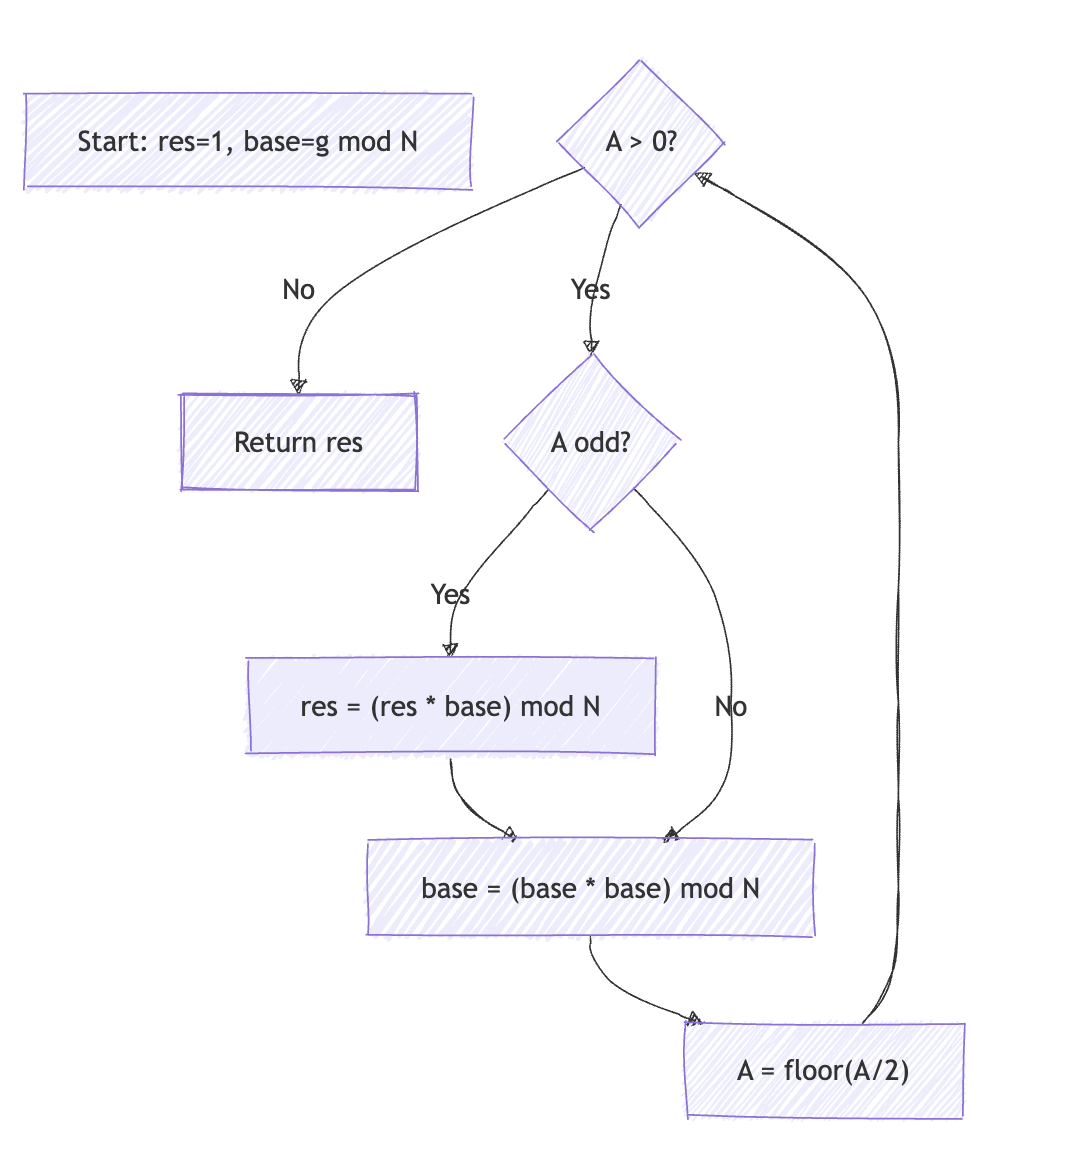
\includegraphics[width=\linewidth]{image.png}
\end{center}

\section{Proof of Correctness}

\begin{theorem}
The binary exponentiation algorithm correctly computes $g^A \pmod{N}$.
\end{theorem}

\begin{proof}
We prove by induction on $A$.
\noindent
\\
\textbf{Base Case:} If $A = 0$, then res $= 1$, and $g^0 = 1$. If $A = 1$, one iteration occurs: $A$ is odd, res becomes $1 \cdot g = g$, base is squared (unused), $A$ becomes 0. \text{correct}.
\noindent
\\
\textbf{Inductive Hypothesis:} Assume correctness for all exponents less than $A$.
\noindent
\\
\textbf{Inductive Step:} Write $A = 2B + \delta$ where $\delta = A \bmod 2 \in \{0,1\}$ and $B = \lfloor A / 2 \rfloor < A$.
\begin{itemize}
  \item If $\delta = 1$, we compute res = $1 \cdot g$;
  \item base becomes $g^2$, $A$ becomes $B$;
  \item recursively, we compute $(g^2)^B = g^{2B}$ and multiply by $g$ if $\delta = 1$.
\end{itemize}
\noindent
\\
Therefore:
\[
g^A = 
\begin{cases}
g^{2B}, & \text{if } \delta = 0 \\
g \cdot g^{2B}, & \text{if } \delta = 1
\end{cases}
\]
\noindent
\\
Each operation is done modulo $N$, so modular equivalence is preserved.
\end{proof}

\section{Complexity Analysis}

The loop runs $\lfloor \log_2 A \rfloor + 1$ times (number of bits in $A$).

\begin{itemize}
  \item Each iteration includes 1 squaring (a multiplication).
  \item Additional multiplication if the bit is 1 (up to $\log_2 A + 1$, average is about $\frac{1}{2} \log_2 A$).
\end{itemize}

\noindent
\textbf{Time Complexity:} $O(\log A)$ multiplications. Each multiplication is $O((\log N)^2)$ with schoolbook arithmetic, or faster with advanced methods (e.g., FFT).
\noindent
\\
Thus, total time is $O(\log A \cdot (\log N)^2)$.
\\
\noindent
\\
\textbf{Space Complexity:} $O(\log N)$ to store intermediate values.
\noindent
\\
This allows computing $g^{2^{1000}} \pmod{N}$ in seconds on modern hardware.

\section{Variants}

\subsection{Sliding Window Method}

For large exponents, the exponent is scanned in $k$-bit windows:

\begin{itemize}
  \item Precompute $g^0, g^1, \dots, g^{2^k - 1}$.
  \item Scan exponent $A$ in $k$-bit windows from most to least significant.
  \item Square $k$ times per window; multiply by precomputed value.
\end{itemize}
\noindent
\\
This reduces the number of multiplications to approximately $(1 + \frac{1}{k}) \log_2 A$.
\noindent
\\
Optimal window size is roughly $k \approx \log \log A$.
\noindent
\\
This is efficient for fixed-base scenarios like RSA public exponentiation.

\subsection{Montgomery Multiplication}

Montgomery multiplication transforms numbers into a special form:

\[
x \mapsto xR \pmod{N}, \quad \text{where } R \text{ is typically } 2^k > N
\]
\noindent
\\
In this form, multiplications avoid costly divisions by $N$, using only shifts and additions.
\noindent
\\ \\
Montgomery form is ideal for repeated modular multiplications, as used in modular exponentiation.


\chapter{Advanced Topics}

\section{Addition Chains}

Addition chains provide efficient methods to compute large powers with minimal multiplications by building sequences where each element is a sum of two previous elements.

\begin{definition}
  An \textbf{addition chain} for an integer $n$ is a sequence:
  \[
    a_0=1, a_1, a_2, \ldots, a_k = n
  \]
  such that each $a_i$ for $i > 0$ can be written as $a_i = a_j + a_m$ for some $j, m < i$.
\end{definition}
\noindent
\\
Addition chains aim to minimize $k$, the number of multiplications for exponentiation.

\section{Quadratic Residues and Reciprocity}

\begin{definition}
  For an odd prime $p$, an integer $a$ is a \textbf{quadratic residue modulo $p$} if there exists $x$ such that
  \[
    x^2 \equiv a \pmod{p}.
  \]
  Otherwise, $a$ is a \textbf{quadratic nonresidue modulo $p$}.
\end{definition}

\begin{definition}
  The \textbf{Legendre symbol} $\left(\frac{a}{p}\right)$ is defined as:
  \[
    \left( \frac{a}{p} \right) = \begin{cases}
      0 & \text{if } p \mid a, \\
      1 & \text{if } a \text{ is a quadratic residue mod } p, \\
      -1 & \text{if } a \text{ is a quadratic nonresidue mod } p.
    \end{cases}
  \]
\end{definition}

\begin{theorem}[Quadratic Reciprocity]
  For distinct odd primes $p$ and $q$,
  \[
    \left( \frac{p}{q} \right) \left( \frac{q}{p} \right) = (-1)^{\frac{p-1}{2} \cdot \frac{q-1}{2}}.
  \]
\end{theorem}

\section{Number-Theoretic Transform}

The Number-Theoretic Transform (NTT) is a finite field analog of the Fast Fourier Transform (FFT), used for polynomial multiplication modulo a prime.

\begin{itemize}
  \item Requires a prime modulus $p$ where $p = k n + 1$ for $n$ a power of 2.
  \item Uses a primitive $n$-th root of unity modulo $p$.
  \item Facilitates convolution via $\text{NTT}^{-1}(\text{NTT}(a)\times \text{NTT}(b))$.
\end{itemize}

\section{Elliptic Curve Exponentiation}

Elliptic curve cryptography relies on exponentiation in groups formed by points on an elliptic curve over finite fields.

\begin{itemize}
  \item The group law on curves gives point addition.
  \item Scalar multiplication $kP = P + P + \cdots + P$ ($k$ times) analogous to exponentiation.
  \item Fast algorithms similar to binary exponentiation apply for scalar multiplication.
  \item Provides stronger security per key length compared to RSA.
\end{itemize}

\end{document}
